\vspace{0.015\textheight}
This chapter gives an overview of the simulation of events from \ppbar collisions. First, a simplified view of a \ppbar collision is presented and concepts related to different aspects of \ppbar collisions are introduced. Next, a more formal introduction to a \ppbar collision is given. Then, the \pythiaText event generator is described together with the scheme used to model the evolution of partons to stable, observable particles. Finally, a brief description of the CDF detector simulation is provided.

\section{The Proton-Antiproton (\ppbar) Collision}
The colliding protons and antiprotons are in the relativistic regime and so are their constituents, the partons. As the two beams pass through one another (in a beam crossing), a parton within a proton from one beam will collide with a parton within an antiproton from the other beam, traveling in the opposite direction. Often, these collisions are inelastic and produce ``soft'' (low momentum) particles. An occasional elastic collision (a hard scatter) may produce new and heavy particles. %This is an overly simplified descriptions of a hard scattering event. Next few paragraphs will explains the intermediate steps in a purely pedagogical manner. The actual understanding of the details in a hard scatter process is limited.

Figure~\ref{fig:ppbar_collision} is an illustration of a typical 2-to-2 parton hard scattering process in a proton-antiproton collision. In a 2-to-2 process, two incoming partons interact and produce two outgoing partons. As the two incoming partons approach each other, they can exchange virtual particles and radiate real particles (for example, gluons and photons). This radiation is termed \newterm{initial state radiation} (ISR). Similarly, outgoing partons can radiate particles and this is termed \newterm{final state radiation} (FSR). The partons from the broken proton and antiproton that did not take part in the hard scatter are called \newterm{spectator partons} and are also referred to as \newterm{beam remnants}. These spectator partons may interact by exchanging gluons and radiating particles to form stable particles. However, these stable particles tend to be softer, which means they have smaller momenta on average. These interactions form the \newterm{underlying event}, which overlaps with the hard scatter process. The underlying event generates particles that are detected in the tracking system and calorimeters. Often, the energy deposited in the calorimeters from the underlying event is indistinguishable from the energy of particles produced in the primary hard scatter.

\begin{figure}[htbm]
 \centering
 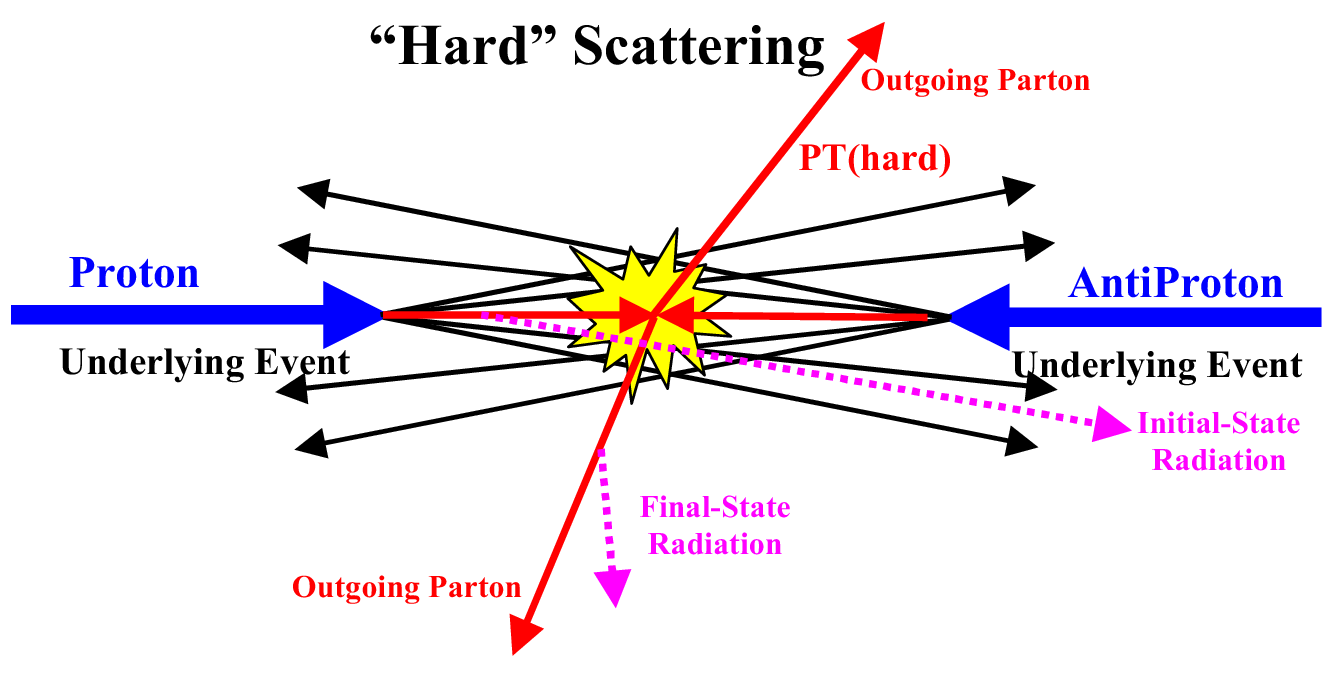
\includegraphics[scale=0.4,keepaspectratio=true]{./ppbar_collision.png}
 % ppbar_collision.png: 1047x528 pixel, 96dpi, 27.70x13.97 cm, bb=0 0 785 396
 \caption{A simulation of a hard 2-to-2 parton scattering process in a \ppbar collision. The \newterm{hard scatter} component consists of the interaction between an incoming parton in the proton and an incoming parton in the antiproton. The interaction produces two outgoing partons (detected as \newterm{jets}), plus ISR and FSR. The \newterm{underlying event} originates from interactions between the remnants of the proton and antiproton.}
 \label{fig:ppbar_collision}
\end{figure}
\vspace{-0.01\textheight}
%Such a event contains particles that originate from the two outgoing partons plus ISR/FSR, and particles from the broken $p$ and $\bar{p}$ (beam remnants).

It is also possible for more than one pair of partons to interact in the same proton-antiproton collision. If two such scattering processes occur, it is \newterm{double-parton scattering}. In this case, it is likely that the second interaction will be quite soft compared to the hard scatter.

Because of the large number of protons and antiprotons circulating in bunches, it is very common to have multiple protons collide with antiprotons in a given bunch crossing. These are known as \newterm{multiple interactions} (MI), and in principle each collision could have a hard scatter. However, in practice, a hard scatter is rare, and multiple interactions usually result in the production of soft particles. Just like the underlying event, particles associated with multiple interactions are difficult to distinguish from the primary hard scatter.

\subsection{Formalism of Hadron Collisions and Perturbative QCD (pQCD)}
\label{sec:pQCD}

The heart of perturbative QCD (pQCD) is the fundamental assumption of asymptotic freedom of the strong coupling constant. Assuming that the strong coupling constant \alphas is small at high-energy (short-distance) interactions, one can approximate such processes by perturbation theory.

QCD provides the formalism to calculate cross sections in high-energy hadron interactions. The cross section for a $2\to2$ hard scattering process (see Fig. \ref{fig:HadHadScattering}) where, for example, a hadron $h$ is produced by $pp \to hX$, can be expressed as:
\begin{eqnarray}
 \frac{d\sigma^{pp\to hX}}{dP} = \sum_{f_{1},f_{2},f} \int dx_{1} dx_{2} dz f_{1}^{p}(x_{1},\mu^{2}_{F}) f_{2}^{p}(x_{2},\mu^{2}_{F}) \nonumber\\*[1.5ex]
 \times \frac{d\hat{\sigma}^{f_{1}f_{2}\to fX^{\prime}}}{dP}(x_{1}p_{1},x_{2}p_{2},p_{h},\mu_{R})\times D_{f}^{h}(z,\mu^{2}_{f})
\end{eqnarray}
where $P$ is any appropriate kinematic variable of the interaction. The quantities $p_{1}$ and $p_{2}$ are the momenta of the initial partons, and $f_{i}^{p}(x_{i},\mu)$ is the probability density function for a parton type $f_{i}$ in the proton to have a momentum fraction $x_{i}$ at a given factorization scale $\mu_{F}$. This is also known as a Parton Distribution Function (PDF). The parameter $\mu_{F}$ is an arbitrary parameter used to avoid singularities in the formulation. There are many different PDF parameterizations, for example CTEQ \cite{pap:CTEQPDF} and MRST \cite{pap:MRSTPDF}. In this analysis, all of the MC samples were generated using the CTEQ5L (leading-order) PDFs. Furthermore, the CTEQ5L PDFs have been compared to MRST PDFs as a way to measure the uncertainty in the CTEQ5L PDFs. Distributions of the PDFs at two different energy scales are shown in Fig.~\ref{fig:PDFsDistributions}.

\begin{figure}[htbm!]
 \centering
 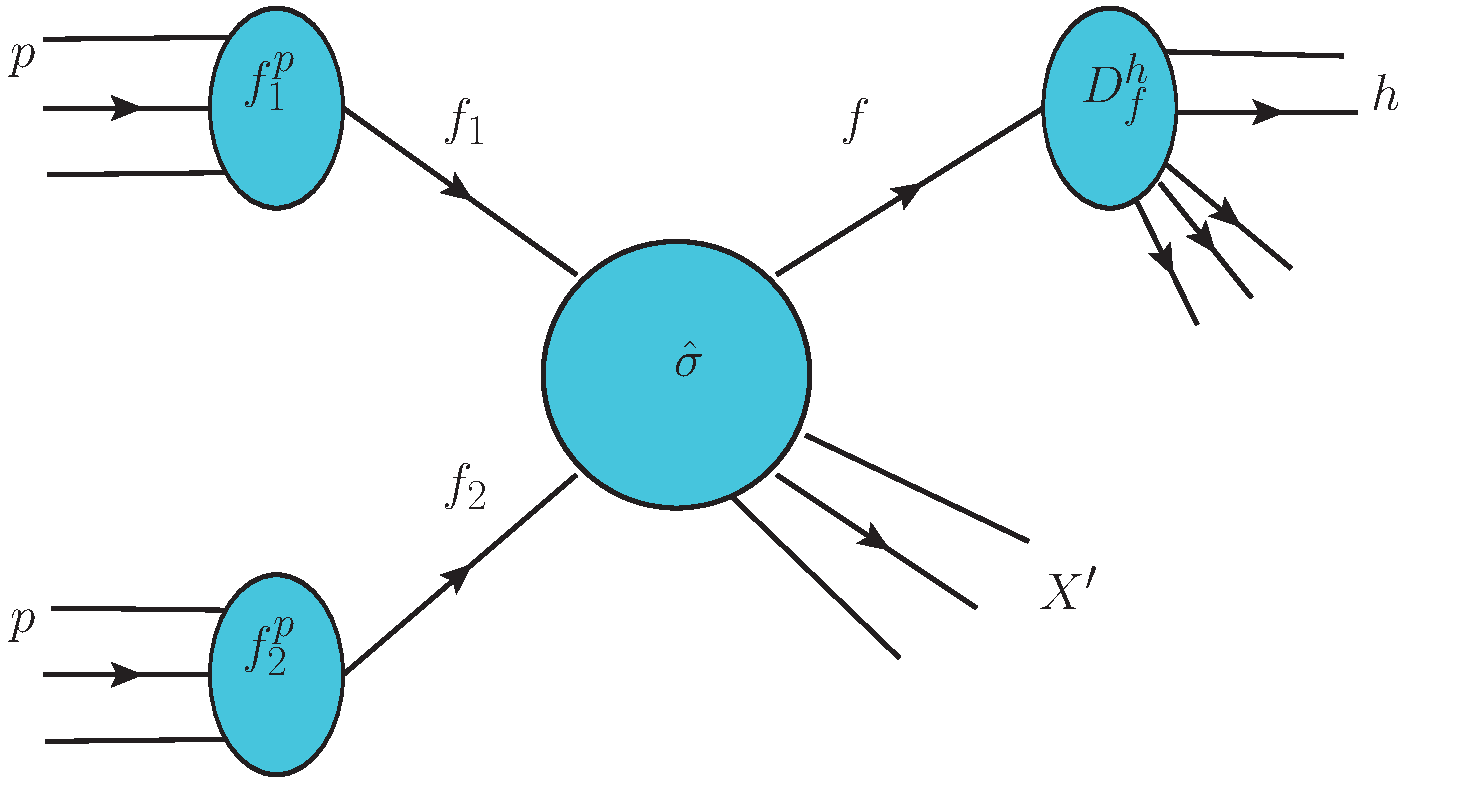
\includegraphics[scale=0.4,keepaspectratio=true]{./hh_collision.pdf}
 % hh_collision.pdf: 711x382 pixel, 72dpi, 25.08x13.48 cm, bb=0 0 711 382
 \caption[Schematic of a $2\to2$ hadron interaction.]{Schematic of a $2\to2$ hadron interaction. The overall interaction is a combination of three parts: the PDFs of the interacting partons, the partonic cross section $\hat{\sigma}$, and the fragmentation of the outgoing partons.}
 \label{fig:HadHadScattering}
\end{figure}

\begin{figure}[p!]
 \centering
 \subfigure[CTEQ5L PDFs]{
 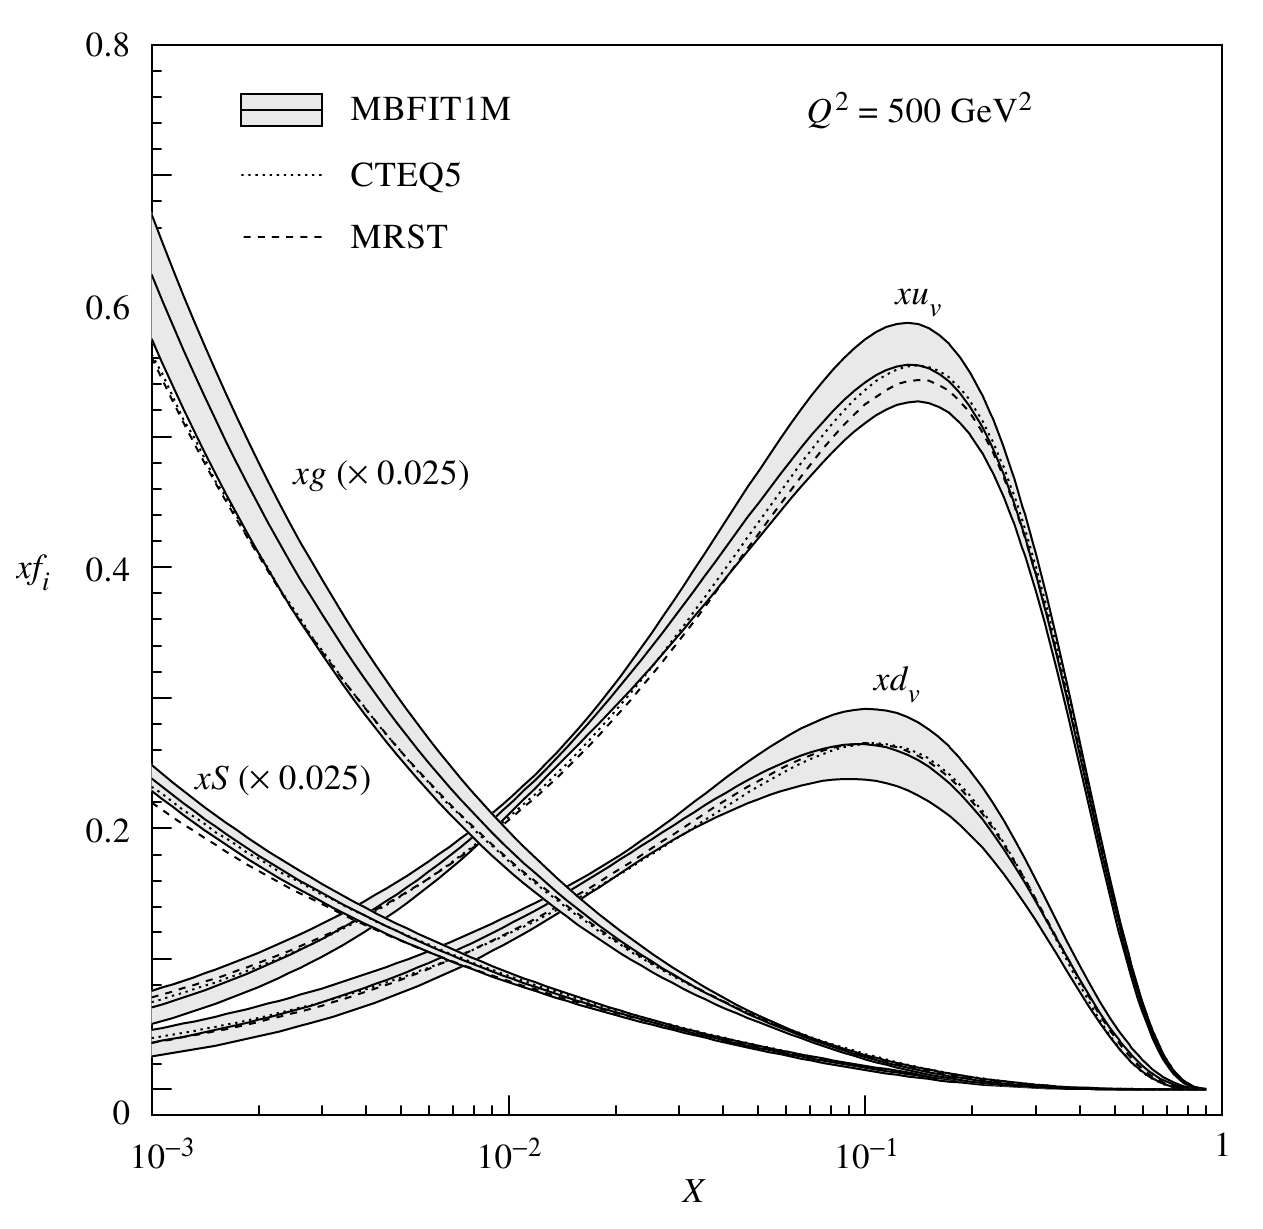
\includegraphics[scale=0.35,keepaspectratio=true]{./CTEQ5PDFs_Distributions.png}
}
\subfigure[CTEQ6M PDFs]{
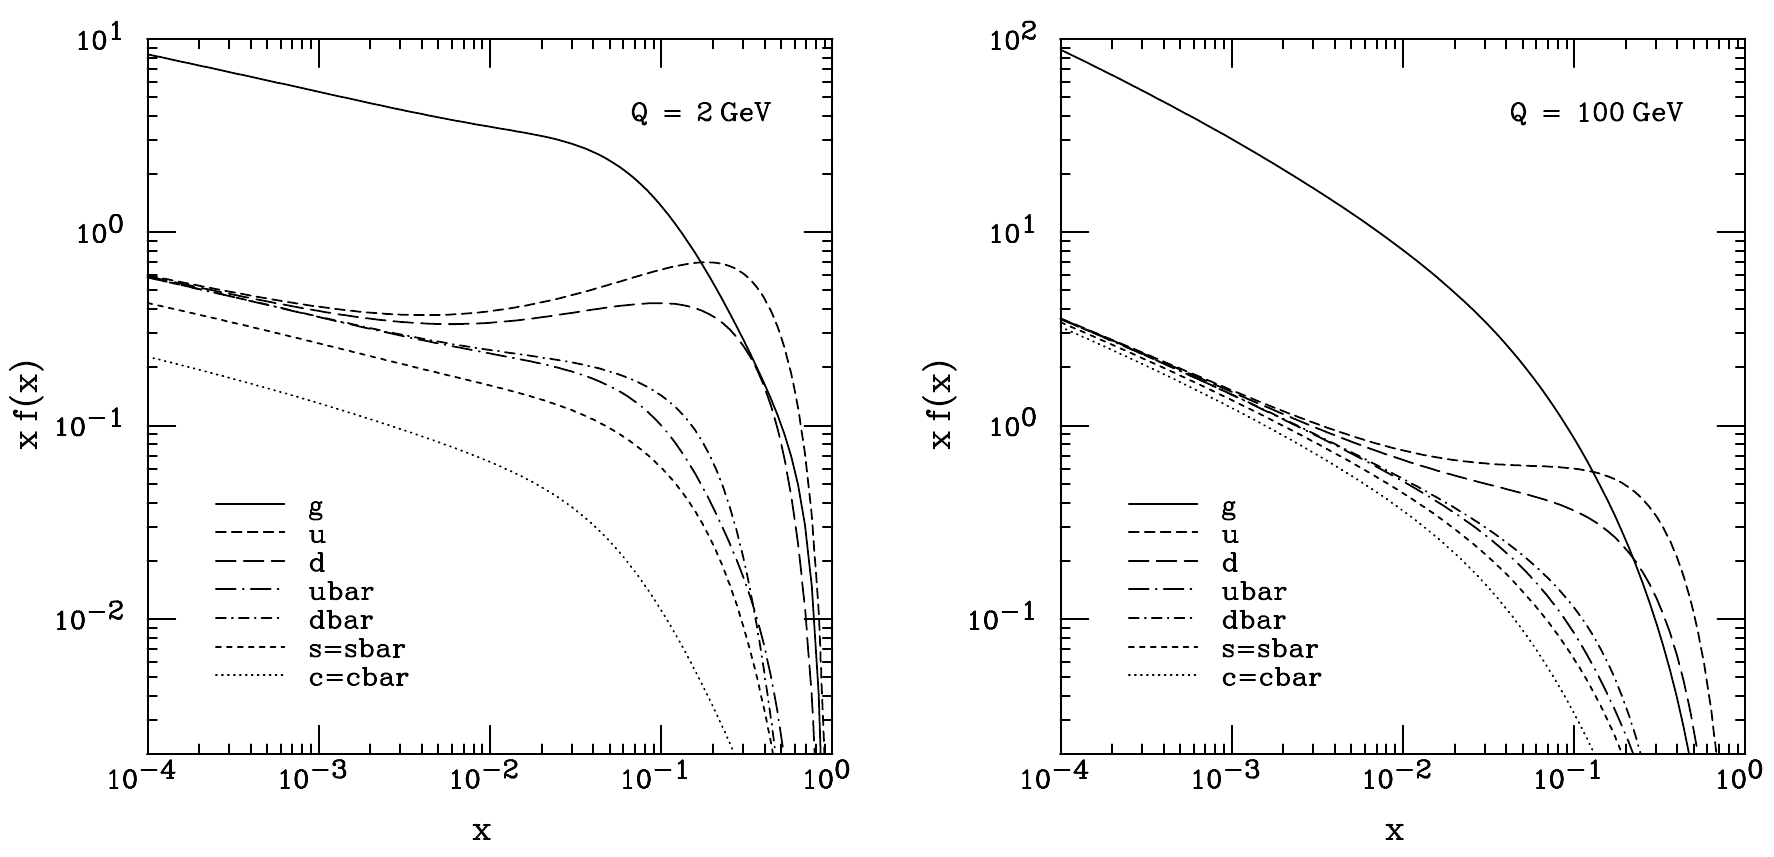
\includegraphics[scale=0.3,keepaspectratio=true]{./PDFs_Distributions.png}
 % PDFs_Distributions.png: 1774x857 pixel, 96dpi, 46.93x22.67 cm, bb=0 0 1330 643
}
 \caption{Overview of parton distributions functions: (a) the CTEQ5L PDFs (leading-order) at $Q^{2}=500$~GeV$^{2}$ \cite{pap:CTEQ5LPDFs} and (b) the CTEQ6M PDFs (next-to-leading order) at $Q=2$ and $Q=100$~GeV \cite{pap:CTEQ6MPDFs}. Several MRST PDFs are overlaid for comparison.}
 \label{fig:PDFsDistributions}
\end{figure}

The quantity $\hat{\sigma}^{f_{1}f_{2}\to fX^{\prime}}$ is the parton cross section calculated at a given order in pQCD and at a renormalization scale $\mu_{R}$. This is the cross section for initial partons with $f_1$ and $f_2$ to produce a final-state parton $f$ and unobserved parton $X^{\prime}$. $D_{f}^{h}(z,\mu^{2}_{f})$ is the fragmentation function, which is the probability density for finding $h$ with fraction of momentum $z$ in the final-state parton $f$ at some fragmentation scale $\mu_f$.

The Factorization Theorem allows one to factorize this total cross section into three parts: the PDF, the parton cross section, and the fragmentation function. This allows the separation of high-energy perturbative processes from low-energy non-perturbative processes. The partonic cross section, $\hat{\sigma}$, can be evaluated perturbatively. But the PDFs ($f_{i}^{p}(x_{i},\mu)$) and fragmentation functions ($D_{f}^{h}(z,\mu^{2}_{f})$) cannot be evaluated perturbatively.

\section{\pythiaText Event Generator}
Event generators, which are based on theoretical calculations, are used to generate physics processes as observed in data. They are used to validate the SM and test for extensions to the SM. There are many different event generators with different capabilities and levels of accuracy. This analysis uses simulated events generated using the \pythiaText Monte Carlo event generator with Tune~A \cite{pap:PythiaManual}. It uses only the leading-order cross section to generate events. \pythiaText simulates the various aspects of a hadron collision: the hard scattering process, the underlying event, and multiple interactions. Then, the different components of the event are overlaid to create the final output.

\pythiaText uses LO matrix element calculations to generate a hard scatter between partons, and it is optimized for $2\to1$ and $2\to2$ scattering processes. Prompt photons are produced in $2\to2$ scattering processes as shown in Fig.~\ref{fig:SM_pj_Feynmans}. Those production process are described in Section~\ref{sec:gjetProdInSM}. Fragmentation, also known as hadronization, is the process whereby partons form colorless hadrons as a result of color confinement. \pythiaText uses \newterm{string} fragmentation. It assumes the quarks are held together by color lines of force that are similar to the electric lines of force between two electric charges as seen in Fig.~\ref{fig:StringFragmentation}. These strings are broken in such a way that color-singlet hadrons are formed out of the vacuum. Fig.~\ref{fig:StringFormation} shows how the strings are formed between partons in the formation of color singlets. This string breaking and formation quickly becomes nonperturbative and extremely hard to calculate. To overcome this difficulty, an object called a \newterm{jet} is defined. By defining a jet, one can ignore the interactions between individual particles (or the higher-order contributions) and avoid the non-perturbative regime altogether. The hadronized particles from a parton will be seen as a collimated spray of particles in the detector. A jet is comprised of charged and neutral particles that are both hadronic and leptonic.

\begin{figure}[htbm!]
 \centering
\subfigure[]{
 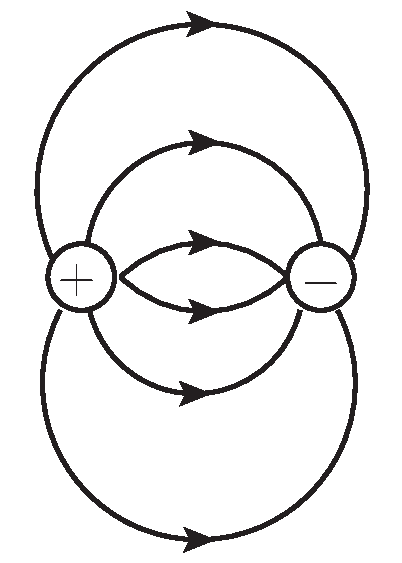
\includegraphics[scale=0.4,keepaspectratio=true]{./LundStringModel.pdf}
}
\subfigure[]{
 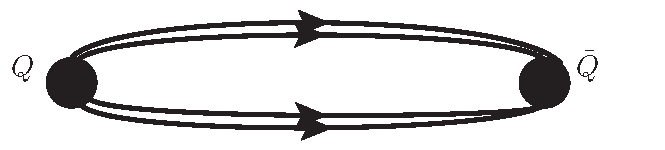
\includegraphics[scale=0.5,keepaspectratio=true]{./LundStringModel2.pdf}
}
\caption{(a) Electric lines of force between two charges. (b) Color lines of force between quarks are pulled together into a tube or string because of the self-interaction between the gluons.}
\label{fig:StringFragmentation}
\end{figure}

\begin{figure}[htbm!]
 \centering
\subfigure[]{
 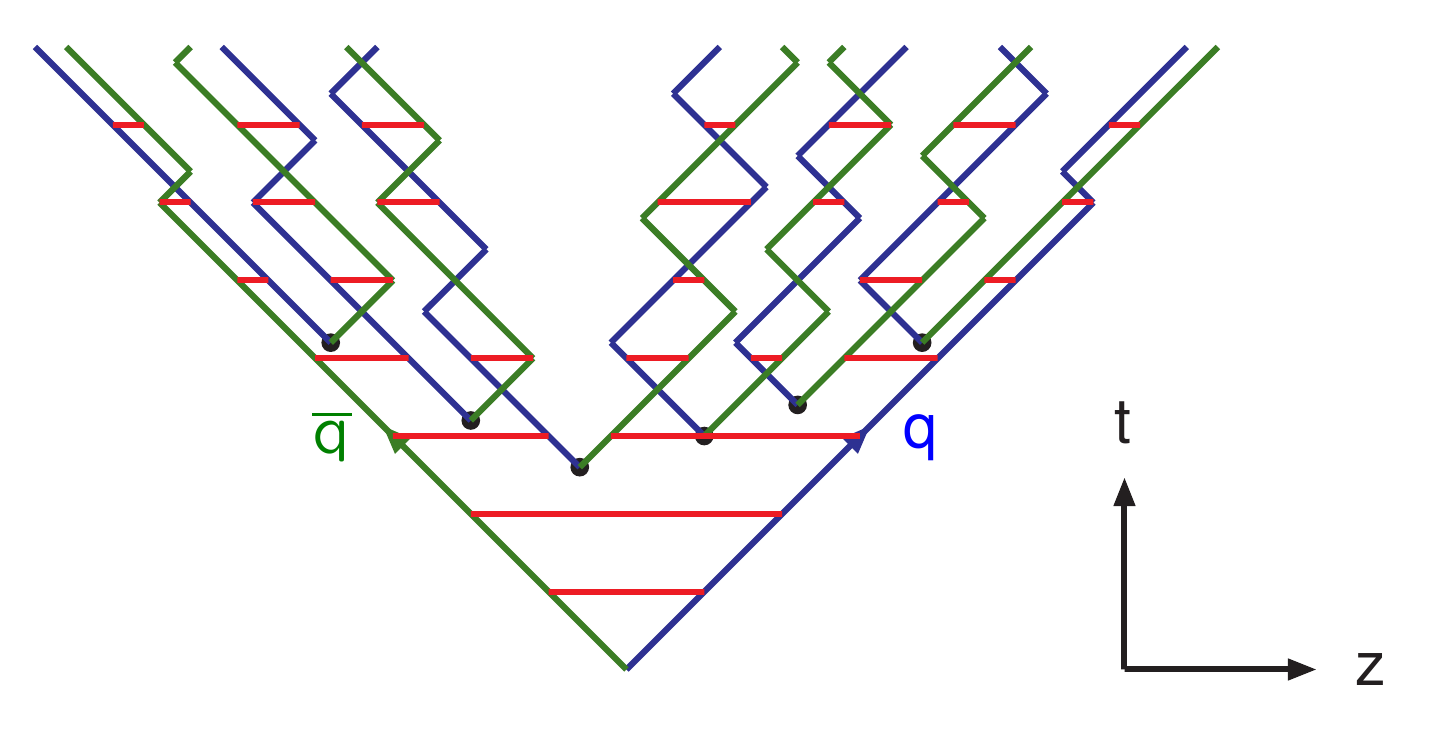
\includegraphics[scale=0.23,keepaspectratio=true]{./StringFormationInQQsystem.png}
}\\
\subfigure[]{
 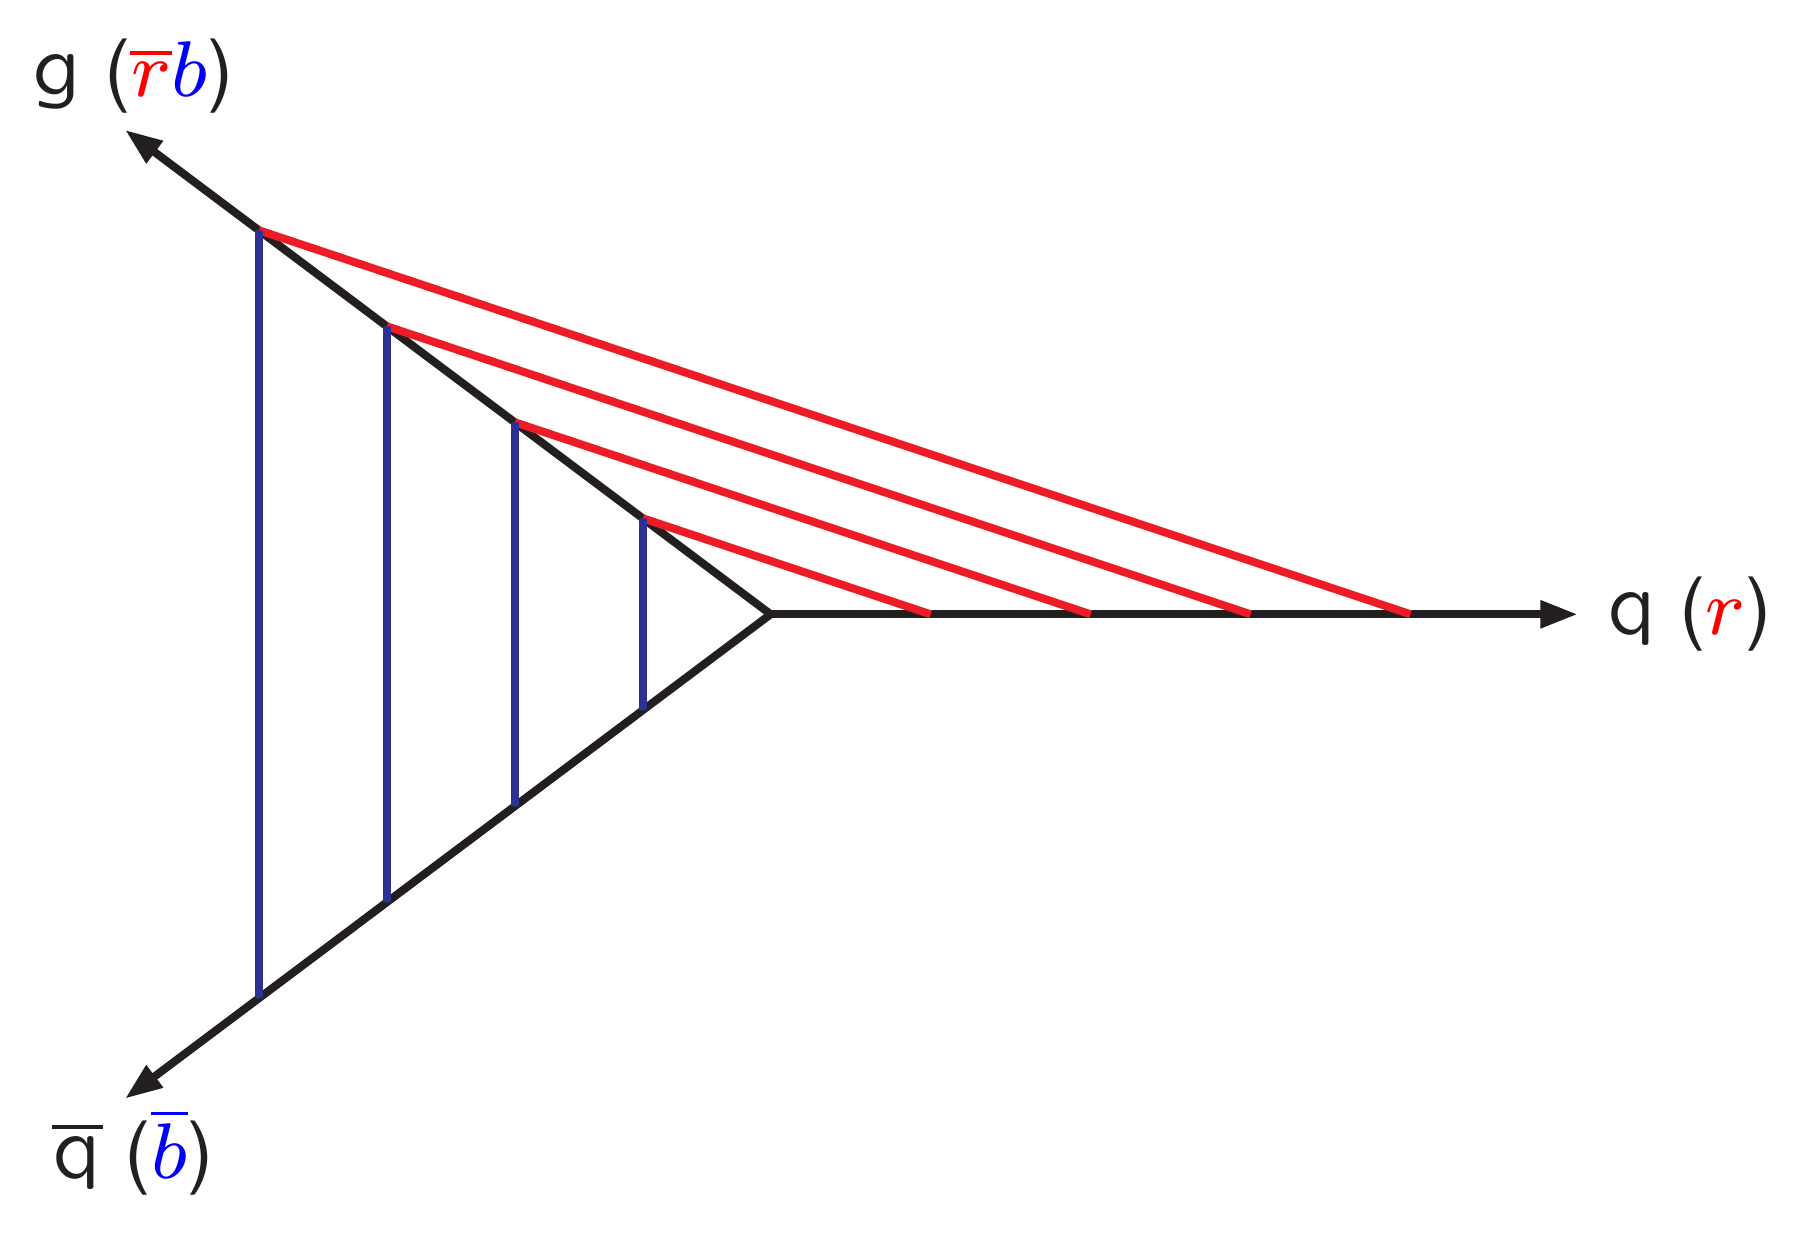
\includegraphics[scale=0.13,keepaspectratio=true]{./StringFormations.png}
}
\subfigure[]{
 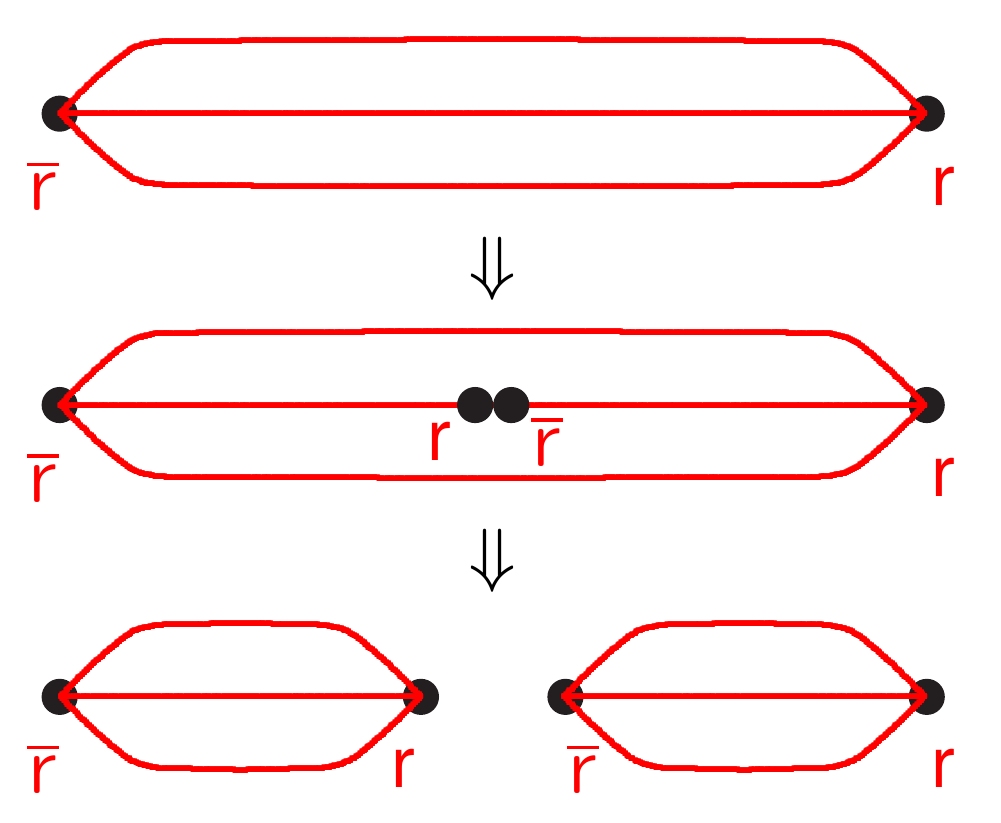
\includegraphics[scale=0.17,keepaspectratio=true]{./StringFormations2.png}
}
 \caption{(a) Overview of hadron production in a $q\bar{q}$ system. (b) Formation of strings between partons. (c) As partons are pulled apart, the potential energy increases and eventually partons are created out of the vacuum to produce colorless hadrons.}
 \label{fig:StringFormation}
\end{figure}

Since \pythiaText cross sections and branching ratios are based on LO calculations they can differ significantly from the theoretical next-to-leading-order (NLO) calculations. As an ad hoc fix to this, LO \pythiaText cross sections are multiplied by a constant factor called a \newterm{$k$-factor}. The $k$-factor is defined by
\begin{equation}
 k=\frac{\sigma(\mbox{NLO})}{\sigma(\mbox{LO})}.
\end{equation}

The $k$-factors can vary depending on how the cross sections are calculated. Cross sections for all of the \pythiaText MC samples used in this analysis have been corrected with a factor of $k=1.4$.

Within \pythiaText, initial-state radiation is computed in backward evolution. Every step in the parton evolution is \pt-ordered and there is an artificial cutoff on the allowed radiation to avoid singularities. Once the parton evolution is complete and stable particles are formed, they are passed into the detector simulation.

%Once an event is generated, minimum bias events are overlaid to improve the modeling of the underlying event and multiple interactions. Minimum bias data are events with no bias from restricted trigger conditions. They include events from nonelastic and diffractive process too. \pythiaText includes only non-diffractive and double-diffractive events in the minimum bias modeling.

\section{Detector Simulation}\label{sec:cdfsim}
A simulation of the CDF detector (\cdfsimText) \cite{www:CDFSIM} is based on a software package called \geantText (GEometry ANd Tracking) \cite{www:GEANT}. \geantText takes into account all the material in the CDF detector as seen in Fig.~\ref{fig:CDFinGEANT}. Every aspect of the detector is carefully accounted for and implemented in the software. The generated particles are tracked by \geantText as they traverse the CDF detector, and secondary physical processes such as energy loss, multiple scattering, and inelastic interactions are simulated. After the first inelastic interaction in the calorimeter, the particles are passed to a program called \gflashText \cite{pap:GFLASH}, which simulates electromagnetic and hadronic particle showers. \gflashText, which uses parameterizations of the calorimeter response, generates particle shower shapes within the calorimeter. The calorimeter parameterization is derived from the response of single particles using test beam data and minimum bias data.

\begin{figure}[htb!]
 \centering
 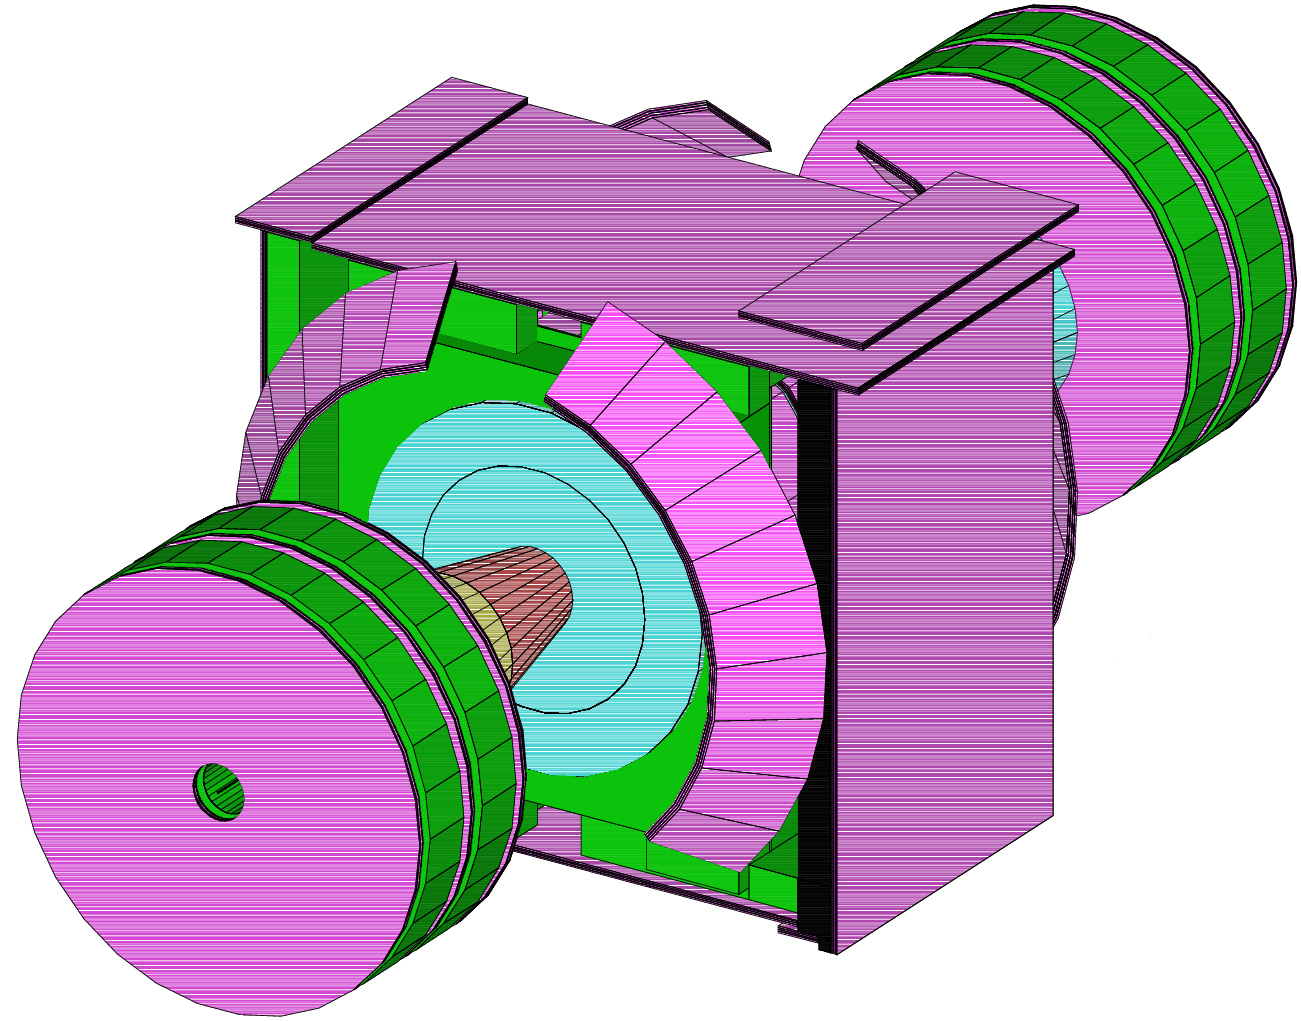
\includegraphics[scale=0.4,keepaspectratio=true]{./CDFinGEANT.png}
 % CDFinGEANT.png: 1301x1021 pixel, 96dpi, 34.42x27.01 cm, bb=0 0 976 766
 \caption{CDF detector volume implemented in \geantText.}
 \label{fig:CDFinGEANT}
\end{figure}


